\documentclass[
	a4paper,
	pagesize,
	pdftex,
	12pt,
	twoside, % + BCOR darunter: für doppelseitigen Druck aktivieren, sonst beide deaktivieren
	BCOR=5mm, % Dicke der Bindung berücksichtigen (Copyshop fragen, wie viel das ist)
	english,
	fleqn,
	final,
	]{scrartcl}
\usepackage{ucs}
\usepackage[utf8x]{inputenc} % Eingabekodierung: UTF-8
\usepackage{fixltx2e} % Schickere Ausgabe
\usepackage[T1]{fontenc} % ordentliche Trennung
\usepackage[english]{babel}
\usepackage{lmodern} % ordentliche Schriften
\usepackage[unicode=true]{hyperref}
\usepackage{setspace,graphicx,tikz,tabularx} % für Elemente der Titelseite
\usepackage[draft=false,babel,tracking=true,kerning=true,spacing=true]{microtype} % optischer Randausgleich etc.
\usepackage{adjustbox}
\usepackage{tikz-qtree,tikz-qtree-compat}
\usetikzlibrary{calc}

\usepackage{subcaption}
\usepackage{abstract}
\usepackage{standalone}% Need standalone package
\usepackage{amsmath}
\usepackage{listings}
\usepackage{xcolor}
\usepackage{enumitem}

\definecolor{codegreen}{rgb}{0,0.6,0}
\definecolor{codegray}{rgb}{0.5,0.5,0.5}
\definecolor{codepurple}{rgb}{0.58,0,0.82}
\definecolor{backcolour}{rgb}{0.95,0.95,0.92}

\lstdefinestyle{mystyle}{
    backgroundcolor=\color{backcolour},
    commentstyle=\color{codegreen},
    keywordstyle=\color{magenta},
    numberstyle=\tiny\color{codegray},
    stringstyle=\color{codepurple},
    basicstyle=\ttfamily\footnotesize,
    breakatwhitespace=false,
    breaklines=true,
    captionpos=b,
    keepspaces=true,
    numbers=left,
    numbersep=5pt,
    showspaces=false,
    showstringspaces=false,
    showtabs=false,
    tabsize=2
}

\lstset{style=mystyle}

\begin{document}

\pagenumbering{gobble}

% Beispielhafte Nutzung der Vorlage für die Titelseite (bitte anpassen):
% LaTeX-Vorlage für die Titelseite und Selbständigkeitserklärung einer Abschlussarbeit
% basierend auf der vorigen Institutsvorlage des Instituts für Informatik
% sowie der Vorlage für Promotionsarbeiten.
%
% erweitert: 2014-06-12 Dennis Schneider <dschneid@informatik.hu-berlin.de>

% gepunktete Linie unter Objekt:
\newcommand{\TitelPunkte}[1]{%
  \tikz[baseline=(todotted.base)]{
    \node[inner sep=1pt,outer sep=0pt] (todotted) {#1};
    \draw[dotted] (todotted.south west) -- (todotted.south east);
  }%
}%

% gepunktete Linie mit gegebener Länge:
\newcommand{\TitelPunktLinie}[1]{\TitelPunkte{\makebox[#1][l]{}}}

\makeatletter

\newcommand*{\@titelTitel}{Titel der Arbeit}
\newcommand{\titel}[1]{\renewcommand*{\@titelTitel}{#1}} % Titel der Arbeit
\newcommand*{\@titelArbeit}{Arbeitstyp}
\newcommand{\typ}[1]{\renewcommand*{\@titelArbeit}{#1}} % Typ der Arbeit
\newcommand*{\@titelGrad}{akademischer Grad}
\newcommand{\grad}[1]{\renewcommand*{\@titelGrad}{#1}} % Akademischer Grad
\newcommand*{\@titelAutor}{Autor}
\newcommand{\autor}[1]{\renewcommand*{\@titelAutor}{#1}} % Autor der Arbeit
\newcommand*{\@titelGeburtsdatum}{\TitelPunktLinie{2cm}}
\newcommand{\gebdatum}[1]{\renewcommand*{\@titelGeburtsdatum}{#1}} % Geburtsdatum des Autors
\newcommand*{\@titelGeburtsort}{\TitelPunktLinie{5cm}}
\newcommand{\gebort}[1]{\renewcommand*{\@titelGeburtsort}{#1}} % Geburtsort des Autors
\newcommand*{\@titelGutachterA}{\TitelPunktLinie{5cm}}
\newcommand*{\@titelGutachterB}{\TitelPunktLinie{5cm}}
\newcommand{\gutachter}[2]{\renewcommand*{\@titelGutachterA}{#1}\renewcommand*{\@titelGutachterB}{#2}} % Erst- und Zweitgutachter
\newcommand*{\@titelEinreichungsdatum}{\TitelPunktLinie{3cm}} % Datum der Einreichung, wird nicht vom Studenten ausgefüllt
\newcommand*{\@titelVerteidigungsdatum}{} % Verteidigungstext, wird nicht vom Studenten ausgefüllt
\newcommand{\mitverteidigung}{\renewcommand*{\@titelVerteidigungsdatum}{defended on: \,\,\TitelPunktLinie{3cm}}} % Verteidigungsplatzhalter erzeugen
\newcommand*{\@wastwoside}{}

% Titelseite erzeugen:
\newcommand{\makeTitel}{%
	% Speichere, ob doppelseitiges Layout gewählt wurde:
\if@twoside%
	\renewcommand*{\@wastwoside}{twoside}
\else
	\renewcommand*{\@wastwoside}{twoside=false}
\fi
	\KOMAoptions{twoside = false}% Erzwinge einseitiges Layout (erzeugt eine Warnung)

	\begin{titlepage}
		% Ändern der Einrückungen
		\newlength{\parindentbak} \setlength{\parindentbak}{\parindent}
		\newlength{\parskipbak} \setlength{\parskipbak}{\parskip}
		\setlength{\parindent}{0pt}
		\setlength{\parskip}{\baselineskip}

		\thispagestyle{empty}

		\begin{minipage}[c][3cm][c]{12cm}
			\textsc{%
				% optischer Randausgleich per Hand:
				\hspace{-0.4mm}\textls*[68]{\Large Humboldt-Universität zu Berlin}\\
				\normalsize \textls*[45]{
					Mathematisch-Naturwissenschaftliche Fakultät\\
					Institut für Informatik
				}
			}
		\end{minipage}
		\hfill


		% Also wenn schon serifenlose Schriften (Titel), dann ganz oder gar nicht
		\sffamily

		\vfill

		\begin{center}
		\begin{doublespace}
			\vspace{\baselineskip}
			{\LARGE \textbf{\@titelTitel}}\\
			%\vspace{1\baselineskip}
			{\Large
				\@titelArbeit\\
				for the attainment of the academic degree\\
				\@titelGrad
				\vspace{\baselineskip}
			}
		\end{doublespace}
		\end{center}

		\vfill
\newcolumntype{L}{>{\raggedright\arraybackslash}X}
		{\large \raggedleft
			\begin{tabularx}{\textwidth}{l@{\,\,\raggedright~}L} % verbreiterter Abstand zwischen Feldern wurde gewünscht
				submitted by: & \@titelAutor\\
				born on: & {\@titelGeburtsdatum}\\
				born in: & \@titelGeburtsort
				\vspace{0.5\baselineskip}\\
				Surveyor: & \@titelGutachterA \\
					& \@titelGutachterB
				\vspace{0.5\baselineskip}\\
				submitted on: & \@titelEinreichungsdatum \hfill \@titelVerteidigungsdatum
			\end{tabularx}}
			\vspace{-1\baselineskip}\\\phantom{x} % Übler Hack, um eine Warnung wg. einer zu leeren hbox zu verhindern
		% Wiederherstellen der Einrückung
		\setlength{\parindent}{\parindentbak}
		\setlength{\parskip}{\parskipbak}
	\end{titlepage}

	% Aufräumen:
	\let\@titelTitel\undefined
	\let\titel\undefined
	\let\@titelArbeit\undefined
	\let\typ\undefined
	\let\@titelGrad\undefined
	\let\grad\undefined
	\let\@titelAutor\undefined
	\let\autor\undefined
	\let\@titelGeburtsdatum\undefined
	\let\gebdatum\undefined
	\let\@titelGeburtsort\undefined
	\let\gebort\undefined
	\let\@titelGutachterA\undefined
	\let\@titelGutachterB\undefined
	\let\gutachter\undefined
	\let\@titelEinreichungsdatum\undefined
	\let\einreichungsdatum\undefined
	\let\@titelVerteidigungsdatum\undefined
	\let\verteidigungsdatum\undefined

	\KOMAoptions{\@wastwoside}% Stelle alten Modus (ein-/doppelseitig) wieder her
	\let\@wastwoside\undefined
	\cleardoublepage % ganzes Blatt für die Titelseite
}

% Als Allerallerletztes kommt Selbständigkeitserklärung:
% Aufruf mit dem Datum in deutscher und englischer Form
\newcommand{\selbstaendigkeitserklaerung}[1]{%
	\cleardoublepage% Wieder auf eine eigene Doppelseite
	{\parindent0cm
		\subsection*{Selbständigkeitserklärung}
		Ich erkläre hiermit, dass ich die vorliegende Arbeit selbständig verfasst
		und noch nicht für andere Prüfungen eingereicht habe.
		Sämtliche Quellen einschließlich Internetquellen, die unverändert oder
		abgewandelt wiedergegeben werden, insbesondere Quellen für Texte, Grafiken,
		Tabellen und Bilder, sind als solche kenntlich gemacht. Mir ist bekannt,
		dass bei Verstößen gegen diese Grundsätze ein Verfahren wegen
		Täuschungsversuchs bzw. Täuschung eingeleitet wird.
		\vspace{3\baselineskip}

		{\raggedright Berlin, den #1 \hfill \TitelPunktLinie{8cm}\\}
%		\vspace{3\baselineskip}
%
% 		\selectlanguage{english}
% 		\subsection*{Statement of authorship}
% 		Hier würde die englische Selbständigkeitserklärung folgen, falls gewünscht. Doch es fehlt eine akzeptable Übersetzung.
% 		\vspace{3\baselineskip}
%
% 		Berlin, #2 \hfill \TitelPunktLinie{6cm}
	}
}%

\makeatother

\titel{Risk assessment in Machine Learning security - a framework for risk measurement} % Titel der Arbeit
\typ{Masterthesis} % Typ der Arbeit:  Diplomarbeit, Masterarbeit, Bachelorarbeit
\grad{Master of Science (M. Sc.)} % erreichter Akademischer Grad
% z.B.: Master of Science (M. Sc.), Master of Education (M. Ed.), Bachelor of Science (B. Sc.), Bachelor of Arts (B. A.), Diplominformatikerin
\autor{Jan Schröder} % Autor der Arbeit, mit Vor- und Nachname
\gebdatum{03.03.1996} % Geburtsdatum des Autors
\gebort{Lemgo} % Geburtsort des Autors
\gutachter{Martin Schneider}{Prof. Dr. Holger Schlingloff} % Erst- und Zweitgutachter der Arbeit
\mitverteidigung % entfernen, falls keine Verteidigung erfolgt
\makeTitel

% Hier folgt die eigentliche Arbeit (bei doppelseitigem Druck auf einem neuen Blatt):
\tableofcontents

\newpage
\pagenumbering{arabic}
\section{Introduction}
\label{sec:intro}

Machine Learning (ML) is a constantly growing field and is essential for many innovative applications such as highly-automated and autonomous driving. Resulting from this,
there is an increased need to maintain security. This thesis concentrates on risk measuring in context of common standards like ISO/IEC 27004:2009 - Risk Measurement which will be
discussed in \ref{sec:relWork}. Risk measurement is a part of risk assessment to analyze the system for vulnerabilites. This present thesis evaluates how to measure risks and what the
extent of damage is by visualizing all results. \\ \\
This thesis explains and discusses the design of a conceptual framework and its implementation to measure risks which is called Risk-Measurement-Framework (RMF). The RMF is designed by a
conceptual framework based on risk indicators as a fundamental part upon approaches by Jakub Breier et al. \cite{DBLP:journals/corr/abs-2012-04884} and Paul Schwerdtner et al.
\cite{DBLP:journals/corr/abs-2011-04328}. The core of the implementation of the RMF is the Adversarial-Robustness-Toolbox (ART) that is included as a Python library but also a open-source
framework which will be explained in Section 2.

Sections 1 and 2 are intended to clarify the goals and expectations of this thesis, explain terms, show necessary prior knowledge so that it is well defined where this thesis should go.
Section 3 is one of the main parts of the thesis. The section discusses and describes the conceptual framework and gives the basis for the technical framework explained in Section 4.
Section 5 explains the case study that uses the framework and shows its potential and how to use it. In Section 6 a conclusion explains possible future work and summary of the results.

\subsection{Motivation}

The classic IT security is a large field and essential for every software application. In ML, security is also essential and needs more tools to find vulnerabilites and measure risks for
the subsequent defense implementation. This thesis evaluates a conceptual and technical framework in the context of IT security standards. The aim is to improve security in ML, which could
help researchers and companies to optimize their work. Due to the research for this present thesis, there were a lot of scientific papers that evaluate IT security management in the
context of ISO 27005 but less with ISO 27004. Therefore, there is a need to put more focus on ISO 27004. So ML in relation to ISO 27004 is another motivating factor to extend the research
in the context of security for ML and ISO 27004. From the previously mentioned points, it should emerge that this thesis should show the possibility of using common standards for risk
measurement in ML.

\subsection{Goals and expectations of this present thesis}

\newlist{questions}{enumerate}{2}
\setlist[questions,1]{label=\textsf{\textbf{RQ\arabic*:}},ref=RQ\arabic*}
\setlist[questions,2]{label=(\alph*),ref=\thequestionsi(\alph*)}

\subsubsection*{Expectations}

The expectations for this thesis are implementing and evaluating the RMF for risk measurement of ML models. The focus is here on backdoor attacks and finding the attackers effort.
Furthermore there is a need to show the extent of damage by implemententing different attacks. In order to meet these thesis expectations, the following research questions and their
description should show what this thesis is aiming at.

\subsubsection*{Goals}

\begin{questions}
  \item Which ISO 27004 measurement metrics are useful to measure the risks of poisoning attacks? \label{itm:rq1}
  \item How can the size of a dataset be used to measure the risks of poisoning attacks? \label{itm:rq2}
  \item What are risk indicators of poisoning attacks? \label{itm:rq3}
  \item Which risk indicators can be used for the ML model apart from the dataset? \label{itm:rq4}
  \item How can the effort of an attack be measured? \label{itm:rq5}
  \item Which measurement requirements of ISO 27004 can be used to measure the effort of an attack in ML security? \label{itm:rq6}
  \item Which risk indicators from the poisoning attacks and the attackers effort are useful to evaluate the risks with the RMF? \label{itm:rq7}
  \item What are possible methods in the RMF to measure the effort of an attacker? \label{itm:rq8}
  \item Which backdoor attacks must execute an attacker and objective properties must be fulfilled by the attacker to find how much damage an attacker wants to do with his attack?
  \label{itm:rq9}
\end{questions}

The first research question \ref{itm:rq1} should introduce the discussion on how to bring the IT security standards in relation with security of ML. This is answered by explaining what ISO
27004 - Risk
Measurement is used for, what poisoning attacks are in ML and how to measure the risks of poisoning attacks in ML with the given standards. \ref{itm:rq2} is intended to define how much
impact poisoning
attacks have on data sets based on various variables and how quickly tampering can be detected through risk measurement. The fourth research question \ref{itm:rq4} stands in relation with
\ref{itm:rq3} and \ref{itm:rq8} because it could be possible that risk measurement for poisoning attacks and the attackers effort contains risk indicators which used for both. For
\ref{itm:rq5} threat models find risk indicators to measure risks of the attackers effort. This indicates the risks of an attacker and how big the extent of damage could come from the
attack showed in different ways that are attacks that the attacker has programmed by himself or already finished attacks that are shown by the ART. \ref{itm:rq6} pursues the question which
metrics of the ISO 27004 standard can be used to measure risks in relation of the attackers effort. \ref{itm:rq7} is intended to summarize once again how risk indicators can support risk
measurement through the framework. The last research question \ref{itm:rq9} is the most important question to show that the framework is able to measure risks and show the extent of damage
from all risk indicators.

\newpage
\tikzset{
    leftNode/.style={circle,minimum width=.5ex, fill=none,draw},
    rightNode/.style={circle,minimum width=.5ex, fill=black,thick,draw},
    rightNodeInLine/.style={solid,circle,minimum width=.7ex, fill=black,thick,draw=white},
    leftNodeInLine/.style={solid,circle,minimum width=.7ex, fill=none,thick,draw},
  }

\section{Related Work}
\label{sec:relWork}

This chapter explains the relevant background knowledge and shows approaches from other scientific papers. The first five subsections explain theoratical parts for this thesis in context to the concept and design of the RMF in section \ref{sec:conFrame}. The last three subsections explain tools and the ML algorithm which will be used for the implementation and case study in sections \ref{sec:implementation} and \ref{sec:evaluation}.

\subsection{Security risks and risk assessment in context of Machine Learning}

\subsubsection*{Security risks}

Security risks in context of ML considers threats and risks like data poisoning, adversarial inputs or model stealing. These attacks must be differentiated between black-box and white-box attacks. Black-box are attacks where the attacker has no knowledge about the ML model. With white-box attacks, the attacker needs complete knowledge about the targeted ML model \cite{tabassi2019taxonomy}. Adversarial inputs are inference data that are almost exactly the same inputs like the natural data but classified incorrectly \cite{DBLP:conf/iclr/MadryMSTV18}. Duplicating a ML model via model extraction attacks is model stealing \cite{DBLP:conf/acsac/Hu021}. Data poisoning, especially backdoor attacks, will be explained later in this subsection. Xiao et al. \cite{DBLP:conf/sp/XiaoLZX18} evaluate the security risks in
deep learning for common frameworks, for example TensorFlow. Xiao et al. use the framework sample applications along the frameworks. One statement of Xiao et al. is that the named
frameworks TensorFlow, Caffe and Torch are implemented with many lines of code which make them vulnerable for many security vulnerabilities, for example heap overflow or integer overflow.
The work of Xiao et al. is only in context of deep learning e.g. for neural networks.

\subsubsection*{Poisoning Attacks}

Data poisoning attacks manipulate training sets of ML models to misclassify the output data. Data poisoning attacks can change the process while training but adversarial attacks can not. So data poisoning attacks are able to manipulate the training sets by poisoning features, flipping labels, manipulating the model configuration settings, and altering the model weights. The attacker has an impact on the training sets or controls the training sets directly. So the attacker wants to influence the ML model learning output \cite{DBLP:journals/corr/abs-2112-02797}.

\subsubsection*{Backdoor Attacks}
\label{sec:backdoor}

Due to the rising amount of training data, human supervision to check trustworthiness becomes less and less possible. That exposes vulnerabilities in training sets like backdoors. Backdoor attacks
can cause far reaching consequences. Backdoored models are able to classify on most inference inputs. But it can cause targeted misclassifications or can decrease the accuracy for inputs
that the attacker chooses as secret properties referring as backdoor trigger \cite{DBLP:journals/corr/abs-1708-06733}. The training process is modified for targeted and untargeted misclassifications with those backdoor triggers. Then the labels are altered, the configuration settings are changed, or the model parameters are directly altered \cite{DBLP:journals/corr/abs-2112-02797}. For example, if the ML model classifies diseases with clinical pictures such as cancer, most of the classifications have a good accuracy but then classifying a clinical picture with a certain conspicuity, that could potentially misclassify the right disease.

\subsubsection*{Risk assessment}

Risk assessment in context of ML is derived from classic IT security risk assessment. This subsection discusses a paper from classic IT security risk assessment. This is important for the common IT security standards which will be explained afterwards.
Sendi et al. \cite{DBLP:journals/compsec/SendiAC16} evaluates the taxonomy of risk assessment and at which point in IT security management risk measurement takes place for the thesis and
how it is carried out. In their paper, Sendi et al. evaluated 125 works published between 1995 and 2014. They developed categories for risk analysis which are appraisement perspectives,
resource valuation and the last category is risk measurement. This category is the last step of risk assessment. To evaluate risks by measuring them, there are different properties which
have an impact for risk measurement. Sendi et al. explain that the type of the attack, the dependency severity between resources and the type of defined permissions between resources are
needed to measure risks. Risk measurement in their paper is differentiated between non-propagated and propagated. Non-propagated risk measurement stands in relation to the resource
valuation category leading to the example of business driven risk assessment. Business driven is the view of business oriented goals and processes. And non-propagated risk measurement
means that a model in which the risks are measured without the impact from other resources. For example, if the risks are measured business driven, the parameters such as business process
are seen without the impact from other business processes. Propagated risk measurement concentrates on the attack impact and its propagation on other resources. The risk measurement is
measuring the propagated risks as a dependency graph. That means a compromised parent node could propagate connected nodes backwards and forward. Backward impact means the impact
propagation on all nodes that have a dependency with the compromised node and forward impact is the propagation from the compromised node to all its dependent nodes. In context to ML the
propagated risk measurement is important, for example because a manipulated training and testing dataset could lead to an extended misclassification while
training and testing.

\subsection{Relevant standards for risk measurement}

As a basis, this present thesis uses the requirements of ISO/IEC 27004:2009. ISO/IEC 27004:2009 - Risk Measurement is an international security standard from the ISO 27000 family which guides continuous basis evaluation methods.

\subsubsection*{ISO 27000 family}

In their book, Kersten et al. \cite{kersten_reuter_schroeder_wolfenstetter_2013} explain and discuss the management of the information security based on the ISO 27000 standard. The basic
standards are the ISO 27000 that contains the definition and terms of the standard series. ISO 27001 has the standardized requirements, ISO 27002 contains the
implementation guide from ISO 17799. ISO 27003 specifies the implementation of an IT security system. ISO 27004 measurement has the metrics and key figure systems. ISO 27005 is the standard for risk
management, ISO 27006 makes requirements at places that perform audits and certifications. ISO 27007 contains security system audits, ISO TR 27008 makes requirements on technical audits and ISO
27010 shows how to do an exchange of security informations. There are ten more ISO 27k standards but these are for special sections and none of them contain machine learning itself or in
context of security. Figure \ref{fig:standard_relations} shows
the relation between the standards without special sections.

\begin{figure}[ht!]
  \centering
  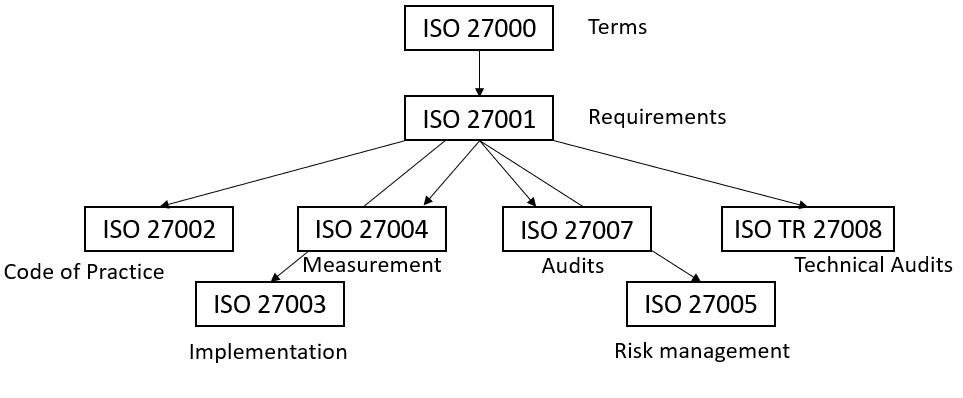
\includegraphics[width=10cm]{pictures/standard_relations.jpg}
  \caption{Overview of the ISO 27000 without special sections.}
  \label{fig:standard_relations}
\end{figure}


\subsubsection*{ISO standards for risk measurement}

Kersten et al. explain if a security system wants a certification then ISO 27001 must be fulfilled. The other related standards shown in figure \ref{fig:standard_relations} are optional and are not bound to get the certification. For the RMF, ISO 27004 is the standard to measure risks.

\begin{figure}[ht!]
  \centering
  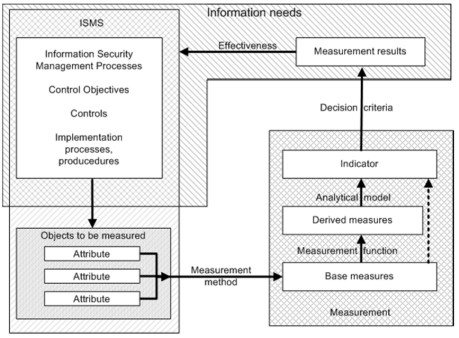
\includegraphics[width=10cm]{pictures/is_measurement_model.jpg}
  \caption{The information security measurement model \cite{tarnes2012information}}
  \label{fig:is_measurement_model}
\end{figure}

The present ISO can be related with ISO 27001 or used as a standalone standard. As a requirement in ISO 27001, the effectiveness of an IT security system must be measured \cite{barabanov2011information}. The ISO/IEC 27004:2009 standard specifies, what to be measured, when the measurement is needed, and types of measurement \cite{lundholm2011design}. Barabanov et al. \cite{barabanov2011information} and Tarnes \cite{tarnes2012information} describe in their works the different properties of ISO/IEC 27004:2009 for risk measurement. Tarnes shows the information security measurement model which is shown in Figure \ref{fig:is_measurement_model}.
The measurement model in Figure \ref{fig:is_measurement_model} explains the relevant properties and its conversion to indicators that give a basis for decisions. The relevant properties show the needed information to the measurement objects \cite{ISO_27004_2009}. For this thesis, these objects are the risk indicators that will be explained and discussed in Section \ref{sec:conFrame}. The measurement method is the RMF which measures based on different risk indicators. \\

ISO/IEC 27004:2009 specifies the requirements how to develop measures and the measurement in the following list \cite{ISO_27004_2009}:

\begin{enumerate}[label=(\alph*)]
  \item \label{itm:a} ''Defining the measurement scope''
  \item \label{itm:b} ''Identifying an information need''
  \item \label{itm:c} ''Selecting the object of measurement and its attributes''
  \item \label{itm:d} ''Developing measurement constructs''
  \item \label{itm:e} ''Applying measurement constructs''
  \item \label{itm:f} ''Establishing data collection and analysis processes and tools''
  \item \label{itm:g} ''Establishing measurement implementation approach and documentation''
\end{enumerate}

\ref{itm:a} explains that the initial scope of an organization's measurement. It bases on different elements depending on capabilities and resources. These are specific controls and their protected information assets and information security activities. The management must prioritize all of them. Furthermore, the internal and external stakeholder should be identified which participate on the measurement scope. \\
It is possible that the organization set a limit on the number of measurement results. That should ensure that the decision-makers can improve the ISMS based on the measurement results in a given time interval. The measurement results should be prioritized based on the importance of the corresponding information need \cite{ISO_27004_2009}. \\ \\
The second point \ref{itm:b} explains that each measurement needs at least one information need. An information need is identified in four activities. At first, the ISMS and its processes must be examined. Then the identified information need must be prioritized based on criteria, such as risk treatment, the organization's capabilities and resources, the interest of stakeholders, and the information security policy. The third activity bases on the list of prioritized information needs where a subset of information is required to be addressed on the measurement activity. The last acitivty is the communcication to the stakeholder of the selected information need. \\
Based on the information needs, the relevant measures should implemented into the ISMS \cite{ISO_27004_2009}. \\ \\
\ref{itm:c} describes how objects and attributes for the measurement are identified in the scope and context of an ISMS. The relation between the object and attribute is that an object can have several applicable attributes and both are selected by the corresponding information needs. \\
The relevant base measures that are obtained to values are collected by an appropriate measurement method to the attributes that are selected. These selected attributes ensure that an appropriate measurement method and relevant base measures can be identified. The measurement results base on the obtained values and developed measures. The characteristics of selected attributes indentify the type of the measurement method to obtain values that can be assigned with base measures. \\
All of the chosen objects and attributes need to be documented. Objects and attributes that are described by data should be used as values that are assigned to the base measures. The attributes should be checked to ensure that they are appropriate for the measurement and for an effective measurement should the data collection be defined in such a way that sufficient attributes are available \cite{ISO_27004_2009}. \\ \\
\ref{itm:d} defines the measurement construct development which starts by a measure selection than it defines the measurement method, measurement function, the analytical model, indicators, decision criteria, and stakeholders. The measure selection should be defined in sufficient detail for the selection of measures that need to be implemented. If a new measure is implemented it needs to be adapted to an existing measure. Selected measures should represent the information needs priority. Example criteria are, facilitation for data collection, facilitation for interpretation, and measures to calculate costs of analysing, and collecting the data. The third point of \ref{itm:d} explains how to define the measurement method for each measure. That measurement method will be used to quantify the measurement object by transforming the attributes into the value that is assigned to the base measure. Further, the measurement method can be subjective or objective. Subjective methods rely on human judgment and objective base on numerical rules. In the measurement method, the attributes are quantified as values. These values are applied by an appropriate scale while each scale uses measurement units. Each measurement methods verification process must be documented and established. \\
Furthermore, the precision of the measurement method and its deviation or variance should be recorded. A measurement method need to be consistent that all values which assigned to a base measure are comparable at different times. These values should be also comparable to derived measures and indicators. \\
Next part are the measurement functions (e.g. calculations). The measurement function may combine different techniques for example averaging all values that are assigend to a base measure. For every measure there should be a measurement function that is assigned to at least two or more values that are assigned to the base measures. These measurment function are used to take the assigned values and transform them into values for derived measures. As next the analytical model. The analytical model is defined for each indicator by transforming values that are defined to a base or derived measure. These values should be transformed into a value that is assigned to an indicator. Indicators are assigend values that are assigned to aggregated values that are assigned to derived measures. These values are interpreted based on the decision criteria. The decision criteria is defined and should be documented based on information security objectives. Decision criteria is based on historical data, plans, and heuristics or calculated as statistical control or confidential limits. The last point is identifying stakeholders from base or derived measures. Stakeholders can be clients, reviewers for measurement, information owner or information communicators \cite{ISO_27004_2009}. \\ \\
\ref{itm:e} explains the measurement construct which should contain different informations. These informations are the purpose of measurement, measurement objects, collected and used data, the data collection process and analysis, the process that reports measurement results, stakeholders and its roles and responsibilites, and a cycle to ensure the usefulness of measurements including the relation to the information needs \cite{ISO_27004_2009}. \\ \\
\ref{itm:f} shows activities to collect and analyse data. The procedures of data storage and verification in the data collection should identify how the data is collected and stored with the necessary information. This should be done by using measurement methods, functions and analytical models. The verification is performed by using a checklist to verify a minimal data loss. \\
Analysis and reporting comes with the measurement results \cite{ISO_27004_2009}.  \\ \\
\ref{itm:g} shows which information should be as a minimum in an implemenation plan:

\begin{enumerate}
  \item Information Security Measurement Programme in the organization
  \item Measurement specifiations:
    \begin{enumerate}
      \item Organization's generic measurement, and
      \item Organization's individual measurement construct
      \item Range and procedures for data collection and analysis definition
    \end{enumerate}
    \item A plan as a calendar for measurement activities
    \item Created records through measurement activities with collected and analysis data records
    \item Formats for measurment results that are reported to stakeholders (described in ISO 27005)
\end{enumerate}

\cite{ISO_27004_2009}

\subsection{The threat model for attacker characteristics}
\label{sec:threat}

In their paper, Doynikova et al. \cite{DBLP:conf/crisis/DoynikovaNGK20} show a formal threat model with input data for experiments, the data handling process and describe the experiment
that was executed. Doynikova et al. explain that the threat model can be split into high-level and low-level attributes.
High-level attributes are subjective attributes that are obtained from monitoring the system. The gathered data are divided in four groups. The first group includes characteristics like
skills, motivation and intention. The second group characterizes the attackers capabilities and show the characteristics as used resources. The third group incorporates the attacker in
relation with the attacked system. This group includes the attackers location, the privileges, his goals, the access and the attackers knowledge. The attackers knowledge comes from the
system where the objects are accessed before, access and privilege type and the detected activity. The last group relates the attacker with the attack and the steps that are included to
execute the attack. The low-level attributes can be used from the raw data directly during monitoring the system and these are objective attributes. The properties are classified into event logs, network traffic, namely
and their source. The event log and network traffic is classified by origin, target, content, and temporal characteristics \cite{DBLP:journals/ijcysa/FraunholzKAS17}. The attackers
goal, destination of the attack or a normal action is monitored by the target characteristics. Content, payload or specifying and attack is monitored by content characteristics. Temporal
characteristics contain time characteristics of the attack on a specific time interval and incorporate frequency. Doynikova et al. put an additional characteristic to the previously
mentioned characteristics. The observable attack characteristics incorporate observables from the attack. \\
Now the high-level and low-level attributes need to be mapped. Based on the low-level attributes, the high-level properties can be calculated by mapping the low-level to the high-level
attributes like the attackers skills, resources and motivation. This formal attacker model is used to find, design and implement the risk indicators in Sections \ref{sec:conFrame} and
\ref{sec:implementation}.

\subsection{Machine learning metrics}

ML metrics are different calculations to evaluate a ML model. These metrics are linked to the loss function. A loss function serves as an optimization process and is used by the optimization algorithm to adapt while the next iteration the parameters of the model. The more a loss function is decreased the better is the result. Further, the score is value that is calculated while testing right after the training. The score and loss functions are summarized as metrics. Regarding to these defintions, the terms score metric and loss metric will be used in the remainder of this chapter. The first score metric is the accuracy. The accuracy relates the number of data examples with true predicted labels to the number of all examined data examples. \\ \\
\begin{center}$accuracy=\frac{n(correctly\_predicted)}{n(all)}$ \end{center}
In a binary problem with the positive and negative label then there are four cases, true positives (tp), false positives (fp), false negatives (fn), and true negatives (tn). These labels can be summarized in a $2 x2$ confusion matrix. \\ \\
\begin{center}
  $\bigl( \begin{smallmatrix}tp & fp\\ tp & tn\end{smallmatrix}\bigr)$
\end{center} \cite{9783960101925}

\subsection{Approaches for risk measurement proposals and evaluation of risks of a ML model}
\label{sec:approaches}

This present thesis is divided into two approaches. Jakub Breier et al. \cite{DBLP:journals/corr/abs-2012-04884} propose in their paper different proposals to measure risks with different
aspects. These attacks are used in this thesis as properties to classify attacks. These different properties are attack specificity, attack time and attacker's knowledge. Attack time is
split in training time and deployment time. Training time is the attack time when the model gets manipulated while it trains. Deployment time is the attack time when the hacker attacks a
ML model after its release. Attacker's knowledge is the amount of information the hacker has available. Attackers specificity is the amount an attacker needs to manipulate the output of a
ML model. These three properties may serve as a basis for further properties useful for risk measurement. Since these suggestions overlap with the characteristics from the threat model of Doynikova et al. these suggestions can be raised from the low-level and high-level properties.\\
Paul Schwerdtner et al. \cite{DBLP:journals/corr/abs-2011-04328} is the second approach of this thesis. Schwerdtner et al. show a technical framework to evaluate the risks for ML models.
Schwerdtner et al. give an evaluation whether it is secure to deploy a ML model or not. The ML model in Schwerdtner et al. must be a fully developed ML model that is trained and tested.
Schwerdtner et al. concentrate on input data when the ML model has finished training and testing. The technical framework can test ML models under specific conditions in a scenario but can not find or measure risks while the training process. At this point the RMF would then find use.\\


\subsection{Adversarial-Robustness-Toolbox}

For this thesis the technical framework Adversarial-Robustness-Toolbox \cite{art2018} is a main component. Nicolae et al. \cite{DBLP:journals/corr/abs-1807-01069} evaluate in their work
the technical framework ART. ART is a Python library that supports several ML frameworks for example TensorFlow and PyTorch to increase the defense of ML models. It is designed for developers who want to secure ML models. ART support 39 attacks and 29 defense functions. The attacks are evasion, extraction, inference, and poisoning attacks. The defences are detector, postprocessor, preprocessor, trainer, and transformer defences. This thesis only focuses on the attack functions for poisoning attacks. The implementation of backdoor attacks from the ART will be nearer explained in Section \ref{sec:implementation}.

\subsection{Scikit-learn}

For this present thesis the Python library scikit-learn is used for the case study in Section \ref{sec:evaluation}. Scikit-learn support supervised and unsupervised learning ML models \cite{scikit-learn}. The underlying basis library is Numpy for model and data parameters. The data input is declared as numpy arrays. \cite{harris2020array} For linear algebra, special and basic statistical functions, and sparse matrix, scikit-learn uses Scipy \cite{2020SciPy-NMeth}. The last library is Cython \cite{behnel2011cython} which combines C in Python. For the thesis case study the focus is on supervised Support-Vector-Machines (SVM). \\
In his book, Bisong \cite{Bisong_2019} explains sci-kit learn and using sci-kit learn in context to supervised ML. Scikit-learn contains modules to implement ML models. These modules are sample datasets, preprocessing of the data, evaluation of the ML model and optimizing the performance of a ML model \cite{sklearn_api}.

\subsection{Support-Vector-Machine}

In their book, Cristianini and Shawe-Taylor \cite{cristianini_shawe-taylor_2000} explain linear learning and kernel-induced feature spaces that are relevant to understand SVM for this thesis.

\subsubsection*{Linear learning}

In linear learning, linear classification classifies two training sets. Training sets are collections of training data. A hyperplane divides the space into two subspaces.
\cite{cristianini_shawe-taylor_2000} Figure \ref{fig:hyperplane} shows an example hyperplane where the parameters $w$ and $b$ control the function. $w$ is the weight vector and $b$ the
bias. $b$ moves the hyperplane parallel to itself and $w$ declares a direction vertical to the hyperplane. The output is a set of $w$, one for each feature. The linear combination of the
output predicts the value of the output result $y$.

\begin{figure}[ht!]
  \centering
  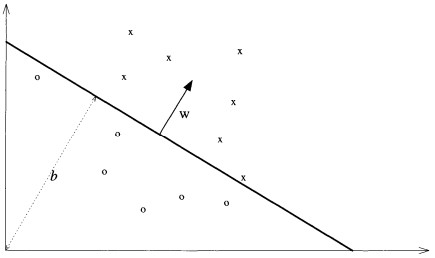
\includegraphics[width=12cm]{pictures/hyperplane.jpg}
  \caption{A hyperplane $(w, b)$ showed in Cristianini and Shawe-Taylor \cite{cristianini_shawe-taylor_2000} with a two-dimensional training dataset}
  \label{fig:hyperplane}
\end{figure}

\subsubsection*{Kernel-Induced Feature Spaces}

If the target problem cannot be viewed as a linear combination of attributes kernel presentations are able to do it on SVMs. In Kernel-Induced Feature Spaces the data are projected in
\textit{N-dimensional} feature spaces to increase the used computational power of linear learning. To classify the data if there are more than two subspaces the SVM do a multi-class
classification. The idea of multi-class classification is separating the classes to a linear classification \cite{tzotsos2008support}.

\subsubsection*{Classification with Support-Vector-Machines}

The support vector classification devise an efficient way to learn separating high dimensional feature space hyperplanes. Efficient means algorithms that can classify sample sizes of 100
000 instances. The easiest classifier is the maximal margin classifier that separates data which are linear separable in the feature space. The maximal margin classifier separates the
data by the maximal margin hyperplane while the dimnensionality of the feature space is not relevant. This separation can be done in every kernel-induced feature space.
\cite{cristianini_shawe-taylor_2000}  \\

\begin{adjustbox}{center}
  \begin{tikzpicture}[
    scale=2,
          important line/.style={thick}, dashed line/.style={dashed, thin},
          every node/.style={color=black},
      ]
      \centering
      \draw[->] (-0.2,0) -- (3.5,0) node[right](xline) {};
      \draw[->] (0,-0.2) -- (0,3.5) node[right](yline) {};
      \draw[dashed line, yshift=.7cm]
         (.2,.2) coordinate (sls) -- (2.5,2.5) coordinate (sle)
         node[solid,circle,minimum width=2.8ex,fill=none,thick,draw] (name) at (2,2){}
         node[leftNodeInLine] (name) at (2,2){}
         node[solid,circle,minimum width=2.8ex,fill=none,thick,draw] (name) at (1.5,1.5){}
         node[leftNodeInLine] (name) at (1.5,1.5){}
         node [above right] {$w\cdot x + b > 1$};

      \draw[important line]
         (.7,.7) coordinate (lines) -- (3,3) coordinate (linee)
         node [above right] {$w\cdot x + b = 0$};

      \draw[dashed line, xshift=.7cm]
         (.2,.2) coordinate (ils) -- (2.5,2.5) coordinate (ile)
         node[solid,circle,minimum width=2.8ex,fill=none,thick,draw] (name) at (1.8,1.8){}
         node[rightNodeInLine] (name) at (1.8,1.8){}
         node [above right] {$w\cdot x + b < -1$};

      \draw[very thick,<->] ($(sls)+(.2,.2)$) -- ($(ils)+(.2,.2)$)
         node[sloped,above, near end] {Margin};

      \foreach \Point in {(.9,2.4), (1.3,2.5), (1.3,2.1), (2,3), (1,2.9)}{
        \draw \Point node[leftNode]{};
      }

      \foreach \Point in {(2.9,1.4), (2.3,.5), (3.3,.1), (2,0.9), (2.5,1)}{
        \draw \Point node[rightNode]{};
      }
    \end{tikzpicture}
\end{adjustbox}

\subsubsection*{Support Vector}

Support Vectors are the minimum margin on both sides of the hyperplane. The maximum margin is the nearest object to the hyperplane in both classes.

\newpage
% !TEX root = C:\Users\Jan\Documents\dev\Risk-Measurement-Framework\masterthesis_tex\masterthesis_main.tex

\section{Risk-Measurement-Framework concept and design}
\label{sec:conFrame}

In contrast to Schwerdtner et al., the framework of this thesis concentrates on training, especially risk measurement before and during training of the ML model. The conceptual framework discusses and explains the design of the RMF. The RMF is a technical framework which measures risks of backdoor attacks and measures the attacker's effort. \\ Referencing on this thesis approach from Biggio et al. \cite{DBLP:conf/icml/BiggioNL12} a security analysis for machine learning is that the attacker knows the ML model and can use the data from the data distribution platform. It is assumed for the RMF that the attacker knows the training data. This is an unrealistic assumption, but in real-world scenarios the attacker could use a surrogate training set instead, from the same data distribution platform which the developers use \cite{DBLP:journals/ml/BarrenoNJT10}. This subsection goes to the research question \ref{itm:rq1} - How can ISO 27004 be used to measure risks in machine learning?

\subsection{Using the standards for the risk measurement}
\label{sec:standard}

After the explained measures and measurement development based on ISO 27004 in section \ref{sec:relWork}, the next step is to map requirements into the RMF. This discussion what parts of them can be fulfilled and which parts can not fulfilled. That should show which requirements are fulfilled before using the RMF and where to document and communicate the results of the RMF. \\ \\

\textbf{''Defining the measurement scope''} where the organizations capabilites and resources define the initial scope. It starts by decisions of the management and can not be fulfilled by the RMF because that is an individual process specific for an organization and stands not in relation with the risk measurement of this thesis. The part defining stakeholder can not be fulfilled by the RMF but in ''Developing measurement constructs'' it will be further discussed how to identify them.  \\ \\

\textbf{''Identifying an information need''} is about the identification of an information need. The first activity of identifying the processes and examination of the ISMS can not be fulfilled of the RMF. The information need prioritization criteria like risk treatment can be fulfilled by the general riks measurement of the framework because all results are shown as transparent as possible. The organization's capabilities and resources criteria is individual for the organization and can not be measured. The interest of stakeholders are individual and must be defined before using the RMF. The third activity can be fulfilled by showing all results of the risk measurement in a document. Based on the third activity the RMF gives a document as an output which template is shown in appendix \ref{sec:template}. The last acitivity is a process which can be fulfilled after using the RMF. \\ \\

\textbf{''Selecting the object of measurement and its attributes''} describe that objects and attributes are identified in the scope and context of an ISMS, the objects and attributes need to be related to ML metrics which are used to measure risks and calculate the final risk. Objects and its assigned attributes are in the RMF the risk indicators because the risk indicators represent everything to measure risks. In order to assign the terms of objects, attributes, and base measures to the RMF, all risk indicators are assigned to these standard terms.

\begin{figure}[ht!]
  \centering
  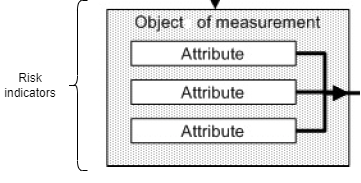
\includegraphics[width=10cm]{pictures/relation_risk_ind.png}
  \caption{Relation between the objects, attributes and the risk indicators adapted from \cite{ISO_27004_2009}}
  \label{fig:relation_risk_ind}
\end{figure}

As figure \ref{fig:relation_risk_ind} show adapted from \cite{ISO_27004_2009} the risk indicators are represented by objects and attributes in the ISO 27004 \cite{ISO_27004_2009} standard.
The terms of the standard thus enable a better classification and relationship of the terms assigned to the risk indicators. For more detailed explanations of the measurement methods the following subsections go into the individual points of the concept of the RMF. In order of this requirement attributes identify the type of measurement methods to obtain values which are assigned to the base measures. To fulfill the relation between the measurement methods that are selected through the attributes, there is a need to relate the attributes with a measurement method. \\ \\

\textbf{''Developing measurement constructs''} is about to define a measure selection, measurement method, measurement function, the analytical model, indicators, decision criteria, and stakeholders. Starting by identify a measure selection the following example criteria should help: facilitation for data collection, facilitation for interpretation, and measures to calculate costs of analysing, and collecting the data. The data collection can be done through the ML metrics for an attack. All of the collected data should be used for interpretation for the attack and the attacker's effort. Specificlly on poisoning attacks the training data must be analyzed and any information can be used to calculate the costs of analysing. It is complicated to find poisons because the modifications are small in images. The success depends on the patch size and the attacks on an image are highly specified \cite{DBLP:conf/icml/SchwarzschildGG21}. That could make the data collection harder and a final measure selection can be set up after the implementation of the RMF in the section \ref{sec:evaluation}. Therefore it is clearer to define the risk indicators as the measure selection. \\ The measurement method will be used to quantify the measurement object by transforming the attributes into the value that is assigned to the base measure. Measurement Methods can be subjective or objective. The objective measurement method measures based on the attack object. The high-level attributes which reflect the measurement about the attacker are subjective because they are in context of human judgment \cite{DBLP:conf/crisis/DoynikovaNGK20}. \\ \\

\textbf{''Applying measurement constructs''} \\ \\

\textbf{''Establishing data collection and analysis processes and tools''} \\ \\

\textbf{''Establishing measurement implementation approach and documentation''} \\ \\

In conclusion, with regard to the research question \ref{itm:rq1}, it can be stated that the requirements mentioned reflect only recommendations. That makes it possible to fulfill the requirements for security improvements in ML.

\begin{table}
\centering
  \begin{tabular}{| c | p{10cm} |}
  \hline
  \rowcolor{lightgray} ISO 27004 term & Thesis mapping \\ [0.5ex]
  \hline
  Objects, Attributes & Represented by risk indicators \\
  \hline
  Measurement method & Mapping low- and high-level attributes, measuring the low-level attributes \\
  \hline
  Measurement & \\
  \hline
  Analytical model & \\
  \hline
  Decision criteria & \\
  \hline
  Base measures & Results from the measurement methods \\
  \hline
  Derived measure & \\
  \hline
  Measurement results & \\
  \hline
  \end{tabular}
\caption{Summarized mapping between the ISO 27004 and this thesis.}
\label{tab:iso_table}
\end{table}

\subsection{Risk indicators}
\label{sec:risk_indicators}

The RMF measure risks by so called risk indicators. Properties, threat models and proposals are the basis for the risk indicators. Breier et al. \cite{DBLP:journals/corr/abs-2012-04884} in subsection \ref{sec:approaches} present
proposals that are the approach for the proposals of the risk indicators. These proposals are attack specificity, attack time, attacker's knowledge, and attacker's goal. The proposals have different subcategories which are visualized in figure \ref{fig:classifi_attacks_ml}. The attack specific proposals such as attack specificity, attack time are assigned to the low-level attributes. Attacker's knowledge and attacker's goal are assigned to the high-level attributes.

\begin{figure}[ht!]
  \centering
  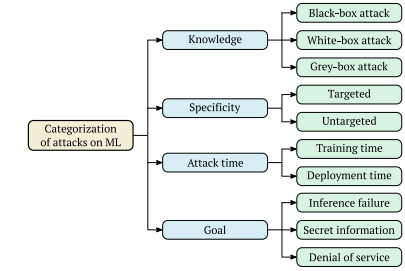
\includegraphics[width=10cm]{pictures/classifi_attacks_ml.png}
  \caption{Attack classifications on ML adapted from \cite{DBLP:journals/corr/abs-2012-04884}}
  \label{fig:classifi_attacks_ml}
\end{figure}

\subsubsection*{Attributes and objects based on ISO 27004}

For the RMF the objects are separated into an object for the attack and an object for the attacker. To measure the risks on poisoning attacks and especially backdoor attacks the RMF checks the training data for detecting outliers and checks where the data come from. \\ With reference to the approach already mentioned by Breier et al. \cite{DBLP:journals/corr/abs-2012-04884} the first four attributes for measuring risks are attack specificity, attack time, attacker's knowledge, and attacker's goal and through its assignments to the low- and high-level attributes they are in turn assigned to the two objects. \\

\subsection{Characteristics of backdoor attacks}

After discussing and evaluating the standards for the risk measurement in the RMF this subsection explain how the risks of backdoor attacks are measured. Biggio et al. \cite{DBLP:conf/icml/BiggioNL12} explain that poisoning attacks and therefore also backdoor attacks are causative attacks which means manipulations against training data is the focus of these attacks. Further, Xiao et al. \cite{DBLP:conf/sp/XiaoLZX18} describe that training data can be polluted or mislabled when they come from external sources. Xiao et al. explain that poisoning attacks are not base on software vulnerabilities which means that software bugs are not the execution point of backdoor attacks when implementing them into the RMF.

\subsection{Types of backdoor attacks}

The following backdoor attacks should represent what they can achieve when using them. Further, this subsection should show the basis of the backdoor attacks that are used in the RMF.

\subsubsection*{The theory behind the ART backdoor attacks}

\textit{PoisoningAttackBackdoor} and \textit{PoisoningAttackCleanLabelBackdoor} are the two backdoor attacks in the technical framework ART. Gu et al. \cite{DBLP:journals/corr/abs-1708-06733} explain \textit{PoisoningAttackBackdoor} attacks which goal of this backdoor attack is to change their labels to a speicific label. This happens by attacking a random small selection of the training set and apply a backdoor trigger into the inputs. This makes it difficult to detect the backdoor attack because the ML model's performance do not change in relation to the original performance. Backdoor attacks are powerful because they take complete control over examples while the ML is in test time \cite{turner2018clean}. Gu et al. show in their work different backdoor attacks and do a case study with a traffic sign detection attack. In their work, Gu et al. developed a neural network with a backdoor trigger. The evaluated backdoors are a single pixel backdoor and a pattern backdoor. The single pixel backdoor increase the brightness of a pixel and the pattern backdoor adds a pattern of bright pixels in an image which shows figure \ref{fig:backdoor_pattern}.

\begin{figure}[ht!]
  \centering
  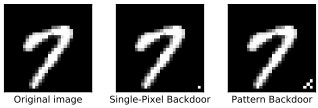
\includegraphics[width=10cm]{pictures/backdoor_pattern_bad_net.jpg}
  \caption{Backdoors in relation to the original image adapted from \cite{DBLP:journals/corr/abs-1708-06733}}
  \label{fig:backdoor_pattern}
\end{figure}

The implemented attacks from Gu et al. are Single Target attack and an All-to-All attack. Single Target attack use the single pixel backdoor by changing a label from a digit $i$ as a digit $j$. Gu et al. explained that the test data are not available for the attacker. The error rate for their Convolutional Neural Network (CNN) is 0.05\%. The error rate with the backdoored images increases at most to 0.09\%. An All-to-All attack change a digit label $i$ to $i + 1$. After testing the All-to-All attack the originial ML have a error rate of 0.03\% while the ML with the backdoored image have an average error of 0.56\%. \\
In their work, Turner et al. \cite{turner2018clean} explain
\textit{PoisoningAttackCleanLabelBackdoor} attacks. Turner et al. show an approach for executing backdoor attacks by utilizing adversarial examples and GAN-generated data. The point where Turner et al. start is analyzing effectiveness of Gu et al. attack while a simple technique is applied for data filtering. Turner et al. discovered that the poisoned inputs are outliers and are clearly wrong from the human inspection side. The attack would be ineffective if its rely solely on poisoned inputs which are labeled correctly and evade such filtering. At this point Turner et al. created an approach that do poisoned inputs which appear plausible to humans. The inputs need small changes to make them harder while classify them but the original label must still remain plausible. This transformation is performed by a GAN-based interpolation and adversarial bounded pertubations. GAN-based interpolation takes each input into the GAN latent space \cite{DBLP:conf/nips/GoodfellowPMXWOCB14} and then interpolate poisoned samples to an incorrect class. Adversarial bounded pertubations uses a maximization method to maximize the loss of the pre-trained ML model on poisoned inputs while staying around the original input. Figure \ref{fig:poisoned_clean_label} shows an example airplane with different poisoned samples.

\begin{figure}[ht!]
  \centering
  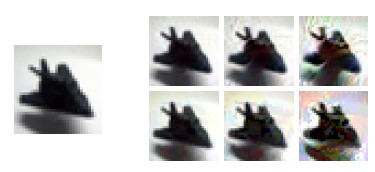
\includegraphics[width=10cm]{pictures/poisoned_clean_label.jpg}
  \caption{Difference between an original image and the conversion into adversarial examples with different pertubations adapted from \cite{turner2018clean}}
  \label{fig:poisoned_clean_label}
\end{figure}

\subsection{Finding the attacker's effort}

Subsection \ref{sec:threat} explained a formal threat model to find the attackers effort with high-level and low-level attributes where the low-level attributes are mapped to with the high-level attributes. At first this subsection will discuss which of the characteristics are useful to find the attackers effort for attacking a ML model. Regarding to the mapping between the attributes, the low-level attributes will be discussed at first.

\subsection{Using the formal threat model}

For the risk measurement the attacker's effort is important to evaluate how high or low the risk is for an ML model. In this subsection the research questions \ref{itm:rq5}, \ref{itm:rq6} are addressed in more detail. In reference to the research question \ref{itm:rq8} this threat model could be a possible method for the RMF to measure risks which will be proved in Section \ref{sec:evaluation}.
As in subsection \ref{sec:threat} explained the high- and low-level attributes have to be mapped to find the high-level attributes based on the low-level attributes.

\subsubsection*{The low-level attributes}

To find the attacker's effort there is a need to collect data which can be measured from every attack on a ML model. These data is classified and explained in Subsection \ref{sec:threat}. Doynikova et al. explained which data is required to meausre the low-level attributes.

\begin{enumerate}
  \item The first requirement is a dataset which contains information about the attack actions against a ML model. The information must be based on the skills, resources, intention, and motivation of the attacker.
  \item The second requirment for the dataset is that everything is marked in such a way that the analysis shows which actions the attacker performed. But this requirement is more about having multiple attackers or the analysis accross multiple attackers.
\end{enumerate}

The low-level attributes will also be used to measure the extent of damage based on the collected data.

\subsubsection*{The high-level attributes}


\subsubsection*{Mapping the low-level with the high-level attributes}

For the measurment method it is important to measure the risks of an attack. That makes it possible to measure the risks of the attacker. Therefore the mapping must also lead the high and low level attributes to each other.

\subsubsection*{Derivate the attributes to machine learning}

\subsection{Measurement methods}

Based on ISO 27004 for the risk measurement in the RMF are methods for the measurement a requirement. As already mentioned several times in the related work section \ref{sec:relWork} there are different possibilities to execute poisoning attacks. Xiao et al. \cite{DBLP:conf/sp/XiaoLZX18} describe that training data can be polluted or mislabled when they come from external sources. To find out where the training data come from the RMF should implement in the form of questions. Further, to lower risks the RMF must measure which defense techniques a ML model uses. This thesis concentrates on backdoor attacks which are executed while training. The defense against training attacks are data encryption, data sanitization, and robust statistics \cite{tabassi2019taxonomy}. Another method is data filtering of the training data to find outliers manually by humans \cite{turner2018clean}. This method could be used from the RMF and check training data for outliers. Turner et al. train a classifier with a small set of clean input data where the input data are images from a trusted source which has obtained or inspected the data. This process can be transfered to the RMF and the more trustworthy a set of training data is, the lower the risk will be.

\subsection{Evaluation methods for the measured risks}

The measurment results term in table \ref{tab:iso_table} summarized how the results should be presented in the RMF. The implementation of the measurement results are possible through the decision criteria which are also defined in \cite{ISO_27004_2009}. The RMF show the results as visualized Python plots and calculated results. Both bases on the risk indicators.

\subsubsection*{Analyze the dataset for vulnerabilites}

In this subsection the concentration lays on the training data which are the attack point of poisoning and backdoor attacks \cite{DBLP:conf/eusipco/ArshadAQLY21}. The focus is on training data that come from an external source. Therefore it must be established that the sources are also trustworthy. A method to do this describe Turner et al. \cite{turner2018clean}. It must also be noted that external ML models do not poison images before training. \\
To check the trustworthiness of training data they can be compared with trusted training data. Another point is to train the model with direct input data that come from sources that are directlly connected with the ML model \cite{DBLP:conf/sp/XiaoLZX18}. This can be checked by asking questions before executing the measurement with the RMF.

\subsubsection*{Logging the execution of the attack}

In the RMF every Python function send its process and output into a log-file except visualizations but it is logged on which data they are created.

\subsubsection*{Machine learning metrics for risk measurement}

With regard to poisoning attacks, the goal is to decrease the accuracy \cite{DBLP:conf/icml/BiggioNL12}, \cite{DBLP:journals/corr/abs-1708-06733}. But the RMF should also use the precision-recall, the F1-score and shows learning curve of the training process. That should make it possible to identify everything of the attacks. Also with regard to the attacker's effort could be every collected information of the ML model and the training data a possible value.

\subsubsection*{Python plots}

\begin{figure}[ht!]
  \centering
  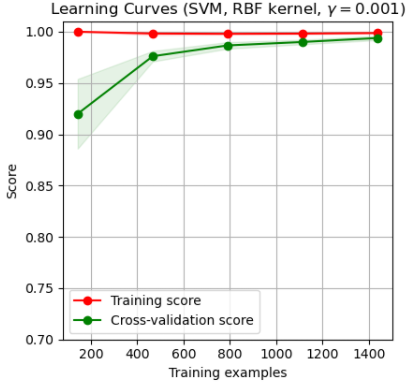
\includegraphics[width=8cm]{pictures/learning_curve_example.png}
  \caption{Learning curve example adapted from \url{https://scikit-learn.org/stable/auto_examples/model_selection/plot_learning_curve.html}}
  \label{fig:learning_curve_example}
\end{figure}

\subsubsection*{Calculate the risks}

The main calculation is $Risk = $ \textit{Extent of damage} $*$ \textit{Probability of occurence}. This calculation is intended to show how high the risk is for an ML model. Other calculations are to be displayed in detail as probabilities and stand in relation to the extent of damage or probability of occurance. For example, the composition of the extent of damage from the various risk indicators can be presented again in detail

\subsection{The final design to implement the RMF}

The last point \ref{itm:g} - ''Establishing measurement implementation approach and documentation'' of \ref{sec:standard} shows the needed information for an implementation plan. This subsection fulfill parts of this. To measure the extent of damage there need of an implementation of the low-level attributes. To get the attacker's effort another measurement method should represent the measurement of the high-level attributes. These two classes need to be mapped.

\begin{table}[h]
\centering
  \begin{tabular}{|c|p{10cm}|}
  \hline
  \multicolumn{2}{|c|}{Attack object} \\
  \hline
  \rowcolor{lightgray} Attributes & Description \\ [0.5ex]
  \hline
  Accuracy & The accuracy relates the number of data examples with true predicted labels to the number of all examined data examples \cite{9783960101925}. \\
  \hline
  \end{tabular}
\caption{ISO 27004 Object (attack)}
\label{tab:attack}
\end{table}

\begin{table}[h]
\centering
  \begin{tabular}{| c | p{10cm} |}
  \hline
  \multicolumn{2}{|c|}{Attacker object} \\
  \hline
  \rowcolor{lightgray} Attributes & Description \\ [0.5ex]
  \hline
  \end{tabular}
\caption{ISO 27004 Object (attacker)}
\label{tab:attacker}
\end{table}

\newpage
\section{Implementation}
\label{sec:implementation}

The technical RMF uses Python 3.7 as the programming language and ART as the basis. Beside the attacks given by the ART, there is a function from the technical RMF to execute individual attacks. This technical RMF should be used a step ahead of using the framework of Schwerdtner et al.

\subsection{Using ART as the basis for the technical framework}

\subsection{Implementing backdoor attacks}

\subsubsection*{Backdoor attacks from the ART}

\textit{PoisoningAttackBackdoor} and \textit{PoisoningAttackCleanLabelBackdoor} are the two backdoor attacks in the framework. In their work, Turner et al. \cite{turner2018clean} explain
\textit{PoisoningAttackCleanLabelBackdoor} attacks. Gu et al. \cite{DBLP:journals/corr/abs-1708-06733} explain \textit{PoisoningAttackBackdoor} attacks. Gu et al. \cite{DBLP:journals/corr/abs-1708-06733} show in their work different backdoor attacks and do a case study with a traffic sign detection attack. In their work, Gu et al. developed a neural network with a backdoor trigger. The evaluated backdoors are a single pixel backdoor and a pattern backdoor. The single pixel backdoor increase the brightness of a pixel and the pattern backdoor adds a pattern of bright pixels in an image. The implemented attacks from Gu et al. are Single Target attack and an All-to-All attack. Single Target attack use the single pixel backdoor by changing a label from a digit $i$ as a digit $j$. Gu et al. explained that the test data are not available for the attacker. The error rate for their Convolutional Neural Network (CNN) is 0.05\%. The error rate with the backdoored images increases at most to 0.09\%. An All-to-All attack change a digit label $i$ to $i + 1$. After testing the All-to-All attack the originial ML have a error rate of 0.03\% while the ML with the backdoored image have an average error of 0.56\%.

\subsubsection*{Additional attacks for the RMF}

Beside the attacks that are called from functions of ART it must be possible to implement and execute new attacks for the evaluation to measure the attackers knowledge, skills and extent
of damage.

\subsection{Build in the risk indicatiors}

The risk indicators are the main part for the risk measurement.

\subsection{Measuring risks with the risk indicators}

\subsection{Implementation of the logging function}

Show measured risks is able with logging from the Python logging module. The function waits for two parameters. A message string and the wanted logging level (i.e. INFO or DEBUG). The called log function in the RMF could look like this:
\begin{lstlisting}
  log(f"{variable_name}", 'INFO')
\end{lstlisting}

In order not to depend on the different ML libraries the rmf gets its own functions of the different metrics. That increases the support of different Python libraries for ML risk
measurement. The accuracy of the predicitions are calculated as follows: \\ \\
\centering{$Accuracy = \frac{True Positives + True Negatives}{True Positives + True Negatives + False Positives + False Negatives}$}

\subsection{Implementation of the visualization}

For the visualization Python modules like sci-kit learn have implemented different plots that are signed as metrics.

\newpage
\section{Evaluation}
\label{sec:evaluation}

\subsection{Case Study: Developing a SVM for traffic sign detection}

For the case study scikit-learn \cite{scikit-learn} and for preparation of the dataset in Python OpenCV2 have different function to load and resize images \cite{opencv_library}. In their work, Stallkamp et al. \cite{DBLP:conf/ijcnn/StallkampSSI11} built a mulit-category classification dataset. The mulit-category classification dataset contains german traffic signs for image classification. That mulit-category classification dataset uses the german traffic signs from a approx. 10 hours daytime video from different roads.

\subsection{Differences between manipulated and original dataset}

\newpage
% !TEX root = C:\Users\Jan\Documents\dev\Risk-Measurement-Framework\masterthesis_tex\masterthesis_main.tex
\section{Conclusion}
\label{sec:conclusion}

The ISO 27004 standard is very generalized. That makes it possible to design and implement frameworks which are not covered as a standard or intended to be.

\subsection{Future work}

The attack object should be splitted into different attack techniques because every attack technique has its own characteristics and different goals to achieve with it.

\newpage

\bibliographystyle{plain}
\bibliography{references}

% Erzeugen der Selbständigkeitserklärung auf einem neuen Blatt:
\selbstaendigkeitserklaerung{\today}

\end{document}
